\subsection{Blockchain}\label{sec:BlockchainModule}

A blockchain is a peer-to-peer distributed ledger forged by consensus, combined with a system for “smart contracts” and other assistive technologies. Together these can be used to build a new generation of transactional applications that establishes trust, accountability and transparency at their core, while streamlining business processes and legal constraints.

SCM-BP uses Blockchain as a supply chain that track parts and service provenance, ensure authenticity of goods, block counterfeits and reduce conflicts.

To achieve that, Hyperledger Fabric is used. Hyperledger is an open source collaborative effort created to advance cross-industry blockchain technologies. It is a global collaboration, hosted by The Linux Foundation, including leaders in finance, banking, Internet of Things, supply chains, manufacturing and Technology.
Hyperledger Fabric is an enterprise-grade permissioned distributed ledger framework for developing solutions and applications. Its modular and versatile design satisfies a broad range of industry use cases. It offers a unique approach to consensus that enables performance at scale while preserving privacy.

In context of SCM-BP, the Blockchain module consists in a smart contract, chaincode and the ledger. From the application developer’s perspective, a smart contract, together with the ledger, form the heart of a Hyperledger Fabric blockchain system. Whereas a ledger holds facts about the current and historical state of a set of business objects, a smart contract defines the executable logic that generates new facts that are added to the ledger. A chaincode is typically used by administrators to group related smart contracts for deployment, but can also be used for low level system programming of Fabric.

\subsubsection{Smart contract}
Before businesses can transact with each other, they must define a common set of contracts covering common terms, data, rules, concept definitions, and processes. Taken together, these contracts lay out the business model that govern all of the interactions between transacting parties.

A smart contract defines the rules between different organizations in executable code. Applications invoke a smart contract to generate transactions that are recorded on the ledger.

\subsubsection{Chaincode}
Hyperledger Fabric users often use the terms smart contract and chaincode interchangeably. In general, a smart contract defines the transaction logic that controls the lifecycle of a business object contained in the world state. It is then packaged into a chaincode which is then deployed to a blockchain network. Think of smart contracts as governing transactions, whereas chaincode governs how smart contracts are packaged for deployment.

\subsubsection{Ledger}
At the simplest level, a blockchain immutably records transactions which update states in a ledger. A smart contract programmatically accesses two distinct pieces of the ledger – a blockchain, which immutably records the history of all transactions, and a world state that holds a cache of the current value of these states, as it’s the current value of an object that is usually required.

Smart contracts primarily put, get and delete states in the world state, and can also query the immutable blockchain record of transactions.

\begin{itemize}
\item A \textbf{get} typically represents a query to retrieve information about the current state of a business object.
\item A \textbf{put} typically creates a new business object or modifies an existing one in the ledger world state.
\item A \textbf{delete} typically represents the removal of a business object from the current state of the ledger, but not its history.
\end{itemize}

Smart contracts have many APIs available to them. Critically, in all cases, whether transactions create, read, update or delete business objects in the world state, the blockchain contains an immutable record of these changes.

\subsubsection{Implementation Details}\label{sec:Implementation}

Our chaincode is written in Golang and provides all contracts needed to proceed traceability in our application. All contracts for use in chaincode must implement the interface \textit{contractapi.ContractInterface}. 

The first step is to create a JSON config file providing all information about these three items. A configuration file includes \textit{assetId}, a list of actors and a list of ordered steps. Our chaincode processes this file through  \textit{initLedger} and \textit{createNewAsset} functions. Here follows a template for config file:  

\begin{lstlisting}
{
   "AssetId":"assetName",
   "Actors":[
      {
         "actorType":"type",
         "aditionalInfo":[
            {
               "key":"value"
            }
         ]
      }
   ],
   "Steps":[
      {
         "step":"stepName",
         "stepOrder":1,
         "actorType":"actorType"
      }
   ]
}
\end{lstlisting}

Front-end WebApp enables a user to define settings through a Configuration Page, adding these to the configuration file, as shown in Figure~\ref{fig:frontend02}.

%htbp
\begin{figure}[ht]
\begin{center}
  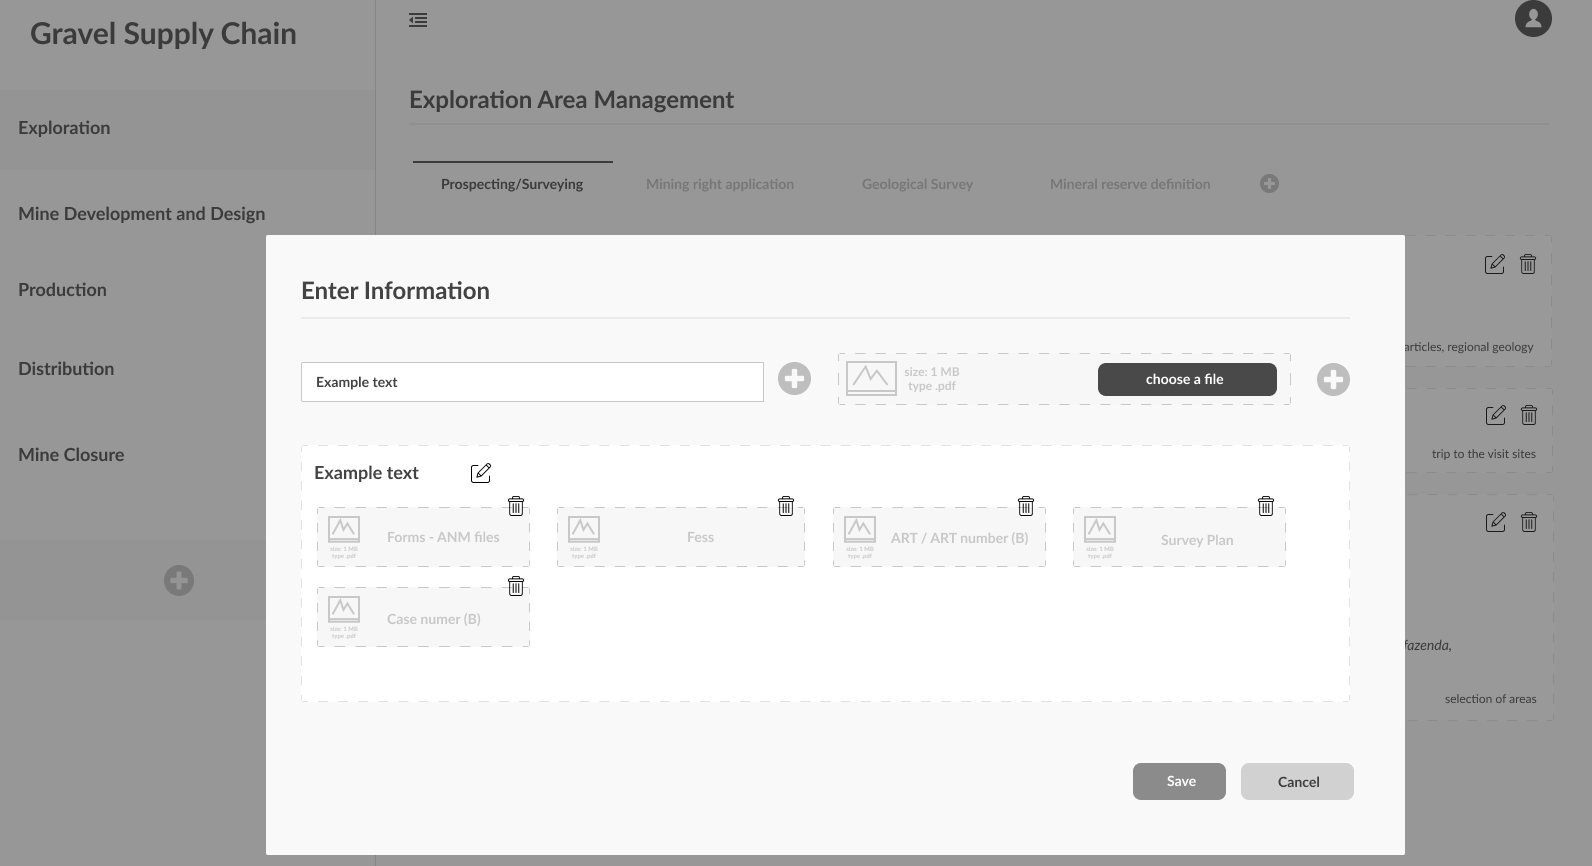
\includegraphics[scale=0.265]{images/frontend02.png}
\caption{SCM Configuration page}
\label{fig:frontend02}
\end{center}
\end{figure}

Assets, asset items, steps and actors are described as \textit{structs}, as follows:

\begin{lstlisting}
type Actor struct {
  ActorId    string  `json:"actorId"`
  ActorType  string  `json:"actorType"`
  ActorName  string  `json:"actorName"`
  AditionalInfo map[string]string `json:"  aditionalInfo"`
}

type Step struct {
  StepId     string  `json:"stepId"`
  StepName   string  `json:"stepName"`
  StepOrder  uint    `json:"stepOrder"`
  ActorType  string  `json:"actorType"`
  AditionalInfo map[string]string `json:"  aditionalInfo"`
}

type AssetItem struct {
  AssetItemId      string  `json:"assetItemId"`
  CurrentOwnerId   string  `json:"currentOwnerId"`
  ProcessDate      string  `json:"processDate"`
  DeliveryDate     string  `json:"deliveryDate"`
  OrderPrice       string  `json:"orderPrice"`
  ShippingPrice    string  `json:"shippingPrice"`
  Status           string  `json:"status"`
  AditionalInfo map[string]string `json:"  aditionalInfo"`
}

type Asset struct {
  AssetId      string       `json:"assetId"`
  AssetItems   []AssetItem  `json:"assetItems"`
  Actors       []Actor      `json:"actors"`
  Steps        []Step       `json:"steps"`
  AditionalInfo map[string]string `json:"aditionalInfo"`
}
\end{lstlisting}

There are create methods for each one,  responsible for creating an instance of these \textit{structs} and save the state into the Blockchain. Query methods are responsible for interact with the information of any item in the Blockchain.


The \textit{main} function of chaincode invokes the \textit{initLedger} function, reads the configuration files and raises the platform enabling users to interact with the Blockchain via exposing its API, as follows: 

\begin{lstlisting}
func main() {
  chaincode, err := contractapi.NewChaincode(
    new(SmartContract)
  )
  if err != nil {
    fmt.Printf("Error create chaincode: %s", err.Error())
    return
  }
  if err := chaincode.Start(); err != nil {
    fmt.Printf("Error starting chaincode: %s", err.Error())
  }
}
\end{lstlisting}

When creating an asset item, an  \textit{AssetItemId} is generated. Each entity in the chain will have its unique entity ID and timestamp when it starts processing the transaction. By querying \textit{AssetItemId}, the user can easily track the current transaction information and status. Finally, completed all steps, the Blockchain will update \textit{deliverDate} and mark the status as completed once the last actor (generally the consumer) has received the order. Here follows \textit{CreateAsset} function:

\begin{lstlisting}
func (s *SmartContract) CreateAsset(
  ctx contractapi.TransactionContextInterface, assetId string, 
  assetItems []AssetItem, actors []Actor, steps []Step, 
  aditionalInfo map[string]string) error {
  
  asset := Asset {
    AssetId:          assetId,
    AssetItems:       assetItems,
    Actors:           actors,
    Steps:            steps,
    aditionalInfo: aditionalInfo,
  }
  assetAsBytes, _ := json.Marshal(asset)
  return 
    ctx.GetStub().PutState("ASSET"+assetId,assetAsBytes)
}
\end{lstlisting}

\textit{ChangeAssetItemOwner} is the method called to update an asset item when it is moved from a step to another. It updates the \textit{CurrentOwnerId}, the \textit{ProcessDate}, information about prices and many other details of the transactions by the key/value map \textit{  aditionalInfo}. Here follows this fuction:

\begin{lstlisting}
func (s *SmartContract) ChangeAssetItemOwner(
  ctx contractapi.TransactionContextInterface, 
  assetItemId string, newOwnerId string, orderPrice string,
  shippingPrice string, status string, 
  aditionalInfo map[string]string) error {
  
  assetItem, err := s.QueryAssetItem(
    ctx, "ASSET_ITEM"+assetItemId)
  if err != nil {
    return err
  }

  assetItem.CurrentOwnerId = newOwnerId
  assetItem.ProcessDate = time.Now()
    .Format("2006-01-02 15:04:05")
  assetItem.OrderPrice = orderPrice
  assetItem.ShippingPrice = shippingPrice
  assetItem.Status = status
  for key, value := range aditionalInfo {
    assetItem.AditionalInfoMap[key] = value
  }
  assetItemAsBytes, _ := json.Marshal(assetItem)
  return 
    ctx.GetStub().PutState(
      "ASSET_ITEM"+assetItemId, assetItemAsBytes)
}
\end{lstlisting}

Figure~\ref{fig:sequenceDiagram} shows the interaction flow from users with Árion platform. Initially, an admin persona creates and configure the SCM, adding information about the steps and the users. After that, the admin can activate this SCM, and from that point, the actors can interact with the SCM to provide information about an asset item and also move this asset item through the supply chain. From that point too, any user can track an asset item to get information about the required good.

%htbp
\begin{figure}[ht]
\begin{center}
  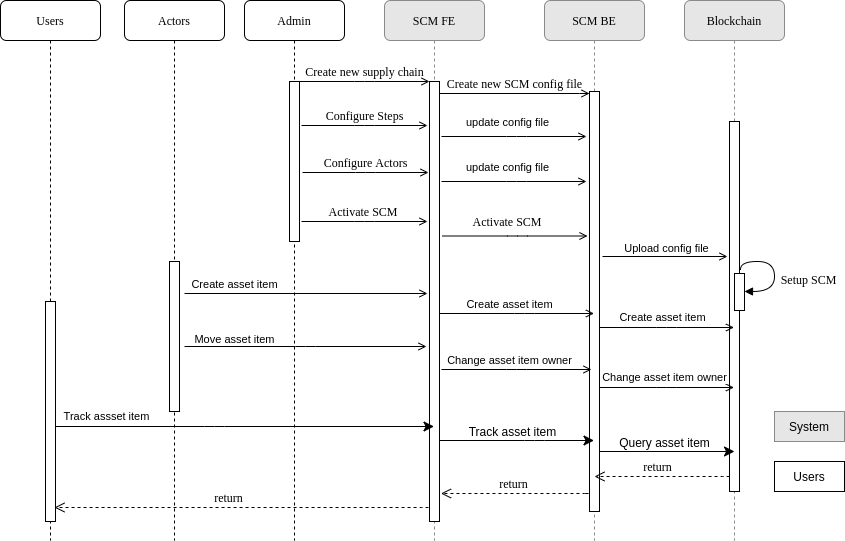
\includegraphics[scale=0.5]{images/SequenceDiagram.png}
\caption{SCM User flow}
\label{fig:sequenceDiagram}
\end{center}
\end{figure}
